\chapter{Authenticating People}

In this class, we will talk a lot about requests
going to a computer system.
And a lot of security comes down to looking at that request and deciding
how to handle it.
For this, it is crucial to know
\textit{who} issued the request. Then, we can
decide whether the system should allow the request. 

Typically, a computer system performs two steps before processing
a request:
\begin{enumerate}
  \item \textbf{Authenticate:} Identify the person 
          or machine (the ``\emph{principal}'') making the request.
  \item \textbf{Authorize:} Decide if the principal 
          is authorized to make the request.
  \item \textbf{Audit:} Log some information about what
          requests your system authorized, so that you can 
          identify malicious requests after the fact and/or
          clean up your system after attacks on the authentication
          system. (For example, a user who accidentally reveals
          their password to an attacker.)
\end{enumerate}

This chapter focuses on authentication.
We will first discuss the attack model and security goals.
Then we will describe common implementations 
that aim to achieve these goals.

\section{Authentication: Security goals}

In the simplest model of authentication, we have a client
and server---two machines communicating over a network.\marginnote{Another
common scenario has a human being authenticating to a computer: think about
typing a PIN into a phone or a password into a computer terminal. We will
discuss this setting more when we come to passwords.}

All authentication schemes try 
to prevent an attacker from impersonating an honest user.
To precisely define the security goal of an authentication
system though, we have to specify the attacker's power:
against which types of attack are we trying to defend?
\begin{figure}
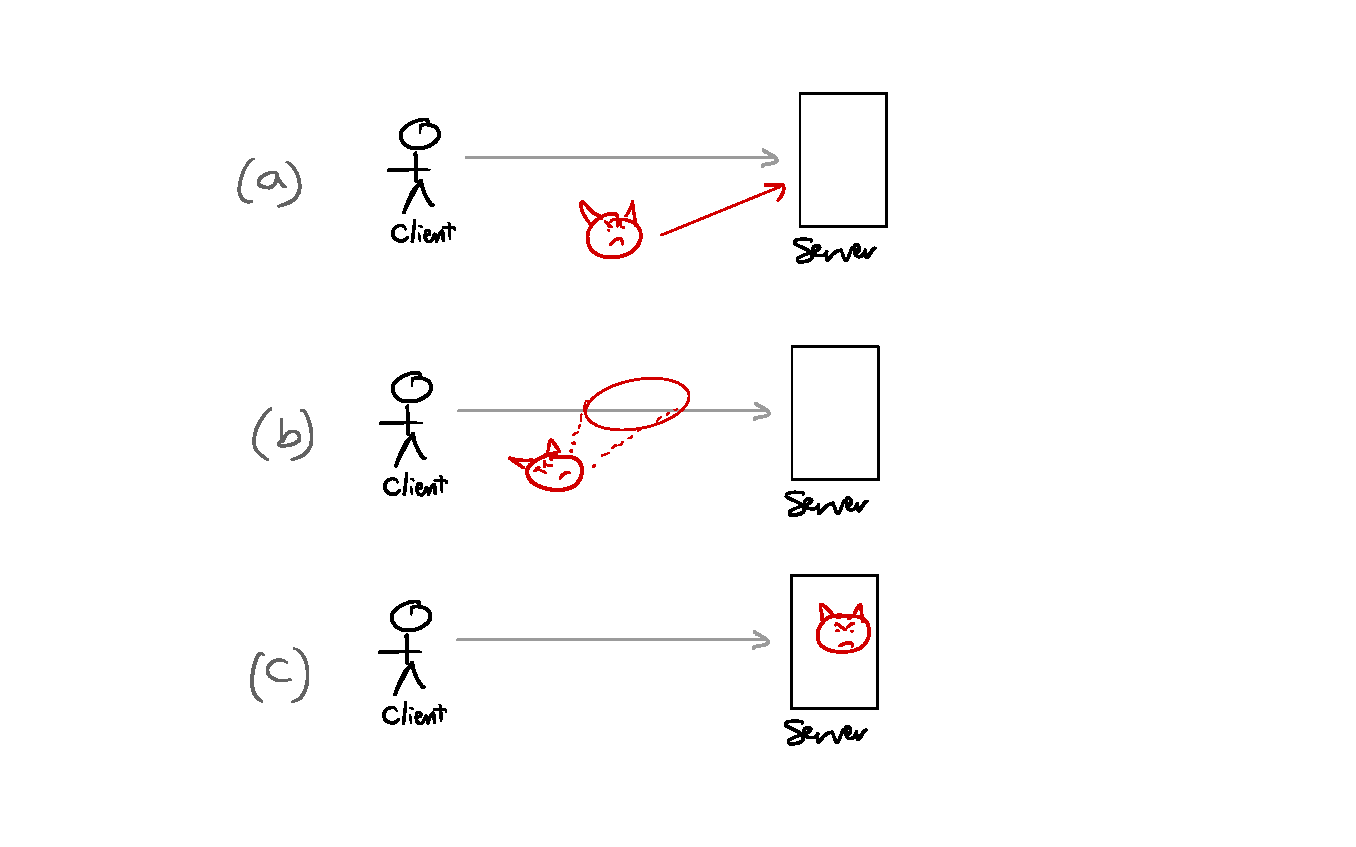
\includegraphics[width=0.9\textwidth]{figs/auth-attacks.pdf}
\caption{There are (at least) three interesting security 
  goals for client-server authentication systems:
  (a) direct attack, (b) eavesdropping attack, and (c) active attack.
}\label{fig:auth-attacks}
\end{figure}


\Cref{fig:auth-attacks} sketches three types of attacks
on authentication systems. In more detail these
are, in increasing order of strength are:
\begin{itemize}
  \item \emph{Direct attack.} 
        The attacker never sees the target user authenticate and then tries
        to impersonate the honest user.
        PIN-based authentication systems, e.g., on your phone or on an ATM
        machine, often aim to defend only against direct attacks.
        The screen-lock password that protects your laptop is also an authentication system
        that just attempts to protect against direct attack.

        That is,
        these systems do not protect against an attacker that can look over your
        shoulder while you are typing your password. These systems only aim to provide
        security when the attacker \emph{never} sees you (the honest user) authenticate.


  \item \emph{Eavesdropping attack.} 
        The attacker observes an honest user authenticating many times---i.e.,
        the attacker sees all of the traffic between the client and server---and then
        tries to impersonate that user.
        One-time passwords, such as the six-digit authentication 
        codes that the Google Authenticator app uses, aim to protect against
        eavesdropping attacks: an attacker who sees one of your one-time passwords
        will not be able to use it to authenticate as you; it is a \emph{one-time} password.

  \item \emph{Active attack.} 
        The attacker that compromises the server, interacts with the honest user,
          and after the server is restored to a good state, tries to authenticate
        as the honest user (\emph{active attack}).

        U2F security keys, and other schemes based on digital
        signatures (\cref{sec:sig}), aim to protect against active attacks.

\end{itemize}
Systems that defend against active attacks provide the strongest
form of security, in that they also protect against eavesdropping attacks
and direct attacks.
Systems that defend against eavesdropping also defend against direct
attacks.
Systems that defend against direct attacks are the weakest---they do not necessarily
provide any protection against the other types of attack.




\section{Protecting against direct attacks:\\ Bearer tokens, PINs, and passwords}

\begin{figure}
\centering
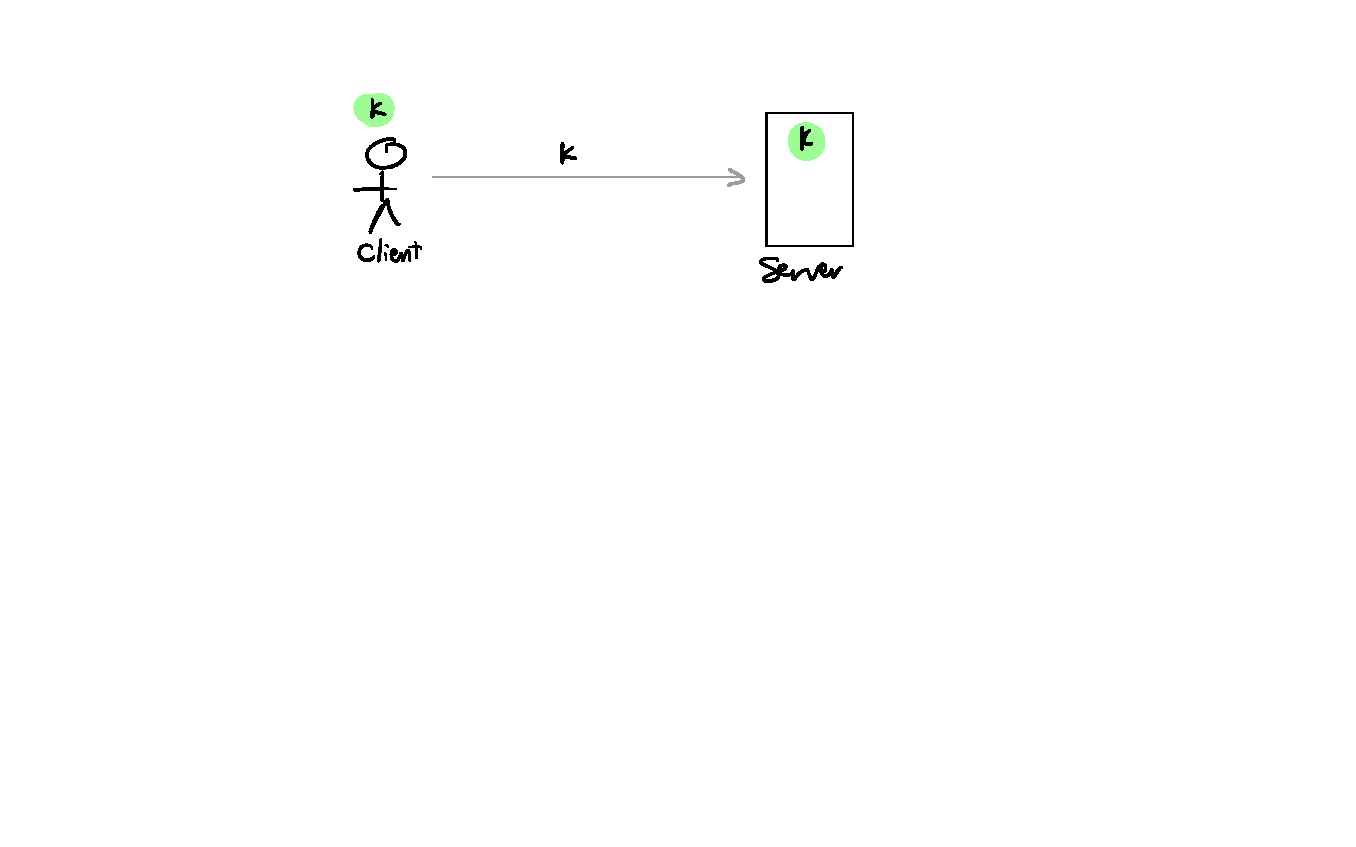
\includegraphics[width=0.7\textwidth]{figs/auth-direct.pdf}
\caption{A bearer-token-based authentication scheme.
To authenticate, the client sends its secret key
$k$ to the server.
{\color{red} WARNING: In practice, the server should store the secret $k$ under
a slow hash function (see \cref{sec:auth:pwhash}).}
}\label{fig:auth-direct}
\end{figure}

The simplest form of authentication uses secret
passwords or PINs. We sometimes call these secret values
\emph{bearer tokens}; whoever bears (holds)
a user's token can authenticate as that user.
Authentication with such schemes works as follows:
\begin{enumerate}
    \item The server holds a password (or PIN or random token string) for the client.
    \item To authenticate, the client sends their password to the server. 
    \item The server checks the password against
          its stored password and accepts if they match.
\end{enumerate}

The benefit of password-based authentication
schemes is that they are simple and easy to implement.
In addition, a human can play the role of the client
in a password-based authentication system (e.g., as you do
when you type a PIN into your phone).
Fancier authentication systems require the client to compute
non-trivial cryptographic functions---not functions that normal
humans can compute in their brains.

Bearer-token-based schemes do provide security against direct attacks:
if an attacker has never seen the user authenticate, the 
attacker's best strategy is to just guess the user's password.
Thus, the security of these schemes against direct attacks depends
entirely on the adversary's uncertainty about the password.

In some bearer-token-based systems, the server can assign
a random password to each user. For example, when you create 
an account for certain web APIs, the API provider 
will give you a random secret key---a bearer token.
You will have to include this secret key with each API request.
Modern APIs use the stronger authentication mechanisms we describe
later in this chapter.

In the vast majority of password- and PIN-based login systems,
the user may choose their own password.
This creates all sorts of headaches\dots

\subsection{What makes a good password?}

\begin{figure}
  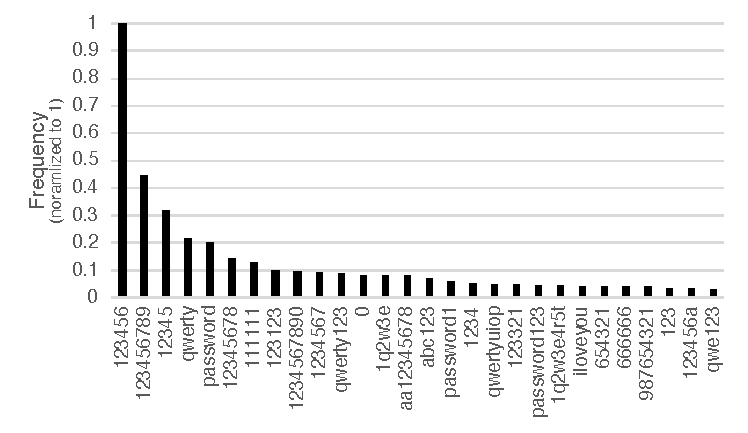
\includegraphics[width=\textwidth]{figs/password-dist.pdf}
  \caption{The most common passwords, according to
  NordPass (\url{https://nordpass.com/most-common-passwords-list/}),
  sorted by their frequency descending.
A small number of common passwords dominate.}
\end{figure}


\marginnote[-2in]{
  \begin{tabular}{cc}
    Rank & Password \\
1 & \ttt{123456}\\
2 & \ttt{123456789}\\
    3 & 12345\\
    4 & qwerty\\
    5& password\\
    6& 12345678\\
    7& 111111\\
    8& 123123\\
    9& 1234567890\\
    10& 1234567\\
    11& qwerty123\\
    12& 000000\\
    13& 1q2w3e\\
    14& aa12345678\\
    15& abc123\\
    16& password1\\
    17& 1234\\
    18& qwertyuiop\\
    19& 123321\\
    20& password123
  \end{tabular}
  \medskip
  \captionof{table}{The most popular passwords in 2021, according to 
  NordPass, \url{https://nordpass.com/most-common-passwords-list/}.}
}

The security of a password-based authentication system
rests entirely on the attacker's inability to guess the password
in a small number of guesses.

\emph{Entropy} is a way to quantify an adversary's
uncertainty about a value sampled using a random
process, or from a particular probability distribution.
If a distribution has $b$ bits of entropy, then
it will take at least roughly $2^b$ guesses 
for an attacker to correctly
guess a value sampled from this distribution.

The uniform distribution over 128-bit strings has 128 bits of entropy.
The distribution from which humans typically choose their passwords
has much less entropy---empirically, more like 20 bits.

Ideally, we would want all passwords to be equally as likely,
from the adversary's perspective.
(These would be ``high-entropy'' passwords.)
If a system generated a truly random password for each user,
each password would be indeed equally likely.
But then it becomes very difficult for a user to remember their 
password, much less many random passwords for many different services.

Typically, people have to remember their passwords,
so we let them pick their own passwords.
When they do,
it turns out that many people are likely to choose
the same password.

A typical password might be sampled from a distribution with roughly
20 bits of 
entropy---if an adversary is able to make $2^{20}$ guesses
at the password, they can expect to guess the password correctly.
One can computer easily make $2^{20}$
authentication requests to another in a few
minutes.

\subsection{Dealing with weak passwords}

\emph{Every} system that uses password- or PIN-based authentication
must contend with the fact that most passwords are not that difficult
for an attacker to guess.

In this section, we describe some mitigation strategies: all are flawed,
but each is better than nothing. The goal of each is to make the attacker's
job slightly more difficult; by stacking a few of these defenses on top
of each other, we can substantially strengthen the end-to-end system.

\paragraph{Aggressively limit the number of guesses.}
Therefore, when using passwords as an authentication
mechanism, an authentication system must \emph{always} 
somehow limit the number of password guesses.

For example, some phones allow 10 guesses at the screen-lock PIN 
before the device resets itself.
Limiting the number of guesses effectively prevents a \emph{single}
account from being compromised---provided that the password is not
too too weak.
One downside is guess limits create the possibility for denial-of-service
attacks: an attacker can potentially make 10 guesses at your password and lock
you out of your phone or online-banking account.

In addition, in many physical computer systems have multiple authorized 
users, each with their own password.
If the guess limit is enforced only on a per-user basis, then an attacker
can often compromise \emph{some} account on the machine if it is allowed
10 guesses at \emph{every} user's password.
Preventing these types of attacks requires some additional measures: websites
that use password authentication rate-limit guesses by IP, or use CAPTCHAs, etc.

\paragraph{Try to coerce users into picking stronger passwords.}
Modern websites will often provide the user with a ``password-strength checker''
that tries to give the user some sense of how strong or weak their password is.
These strength meters are completely heuristic and can be wildly wrong:
they might say that \texttt{6175551212} is a great password; if the attacker
knows that 617-555-1212 is my phone number, it is probably not a great password.
These strength meters sometimes check a user's password against public lists of 
popular passwords. Ensuring that your password isn't in the million most popular
ones gives you at least some protection against untargeted attacks.

Two common strategies for encouraging users to choose strong passwords
that don't work terribly well are:
\begin{itemize}
  \item \emph{Require longer passwords.} If someone tries to use 
    \ttt{abc123} as a password but it's not long
    enough, they might use \ttt{abc123456}---but
    this doesn't really add much uncertainty.
    There are standard ways to lengthen passwords,
    and a clever attacker will try these first.
  \item \emph{Prohibit using common English words in passwords.}
    It's not clear that this is a good idea.
    Five randomly chosen words from the dictionary will
    form a strong password, and prohibiting English words
    in passwords may make passwords much more difficult to remember.

\end{itemize}

\subsection{Avoiding weak passwords with a password manager}
When using passwords to authenticate to a website, 
a user can install a password manager on their
computer that will generate random passwords for them.
Since the user doesn't need to remember these passwords,
they can be sampled truly at random from a high-entropy distribution.
Once the user authenticates to their computer (using a password, typically), 
they can then access their randomly generated passwords and
use them to log in to their websites. 

Internally, the password-manager software maintains a table of 
servers and the corresponding passwords:

\medskip
\begin{tabular}{c|c|c}
  server & user & pw \\ \hline
  \ttt{amazon.com} & \ttt{alice} & \ttt{3xyt42...} \\
  \ttt{mit.edu} & \ttt{alice4} & \ttt{a21\$z...} \\
\end{tabular}
\medskip

Even when using a password manager, password-based authentication
schemes provide \emph{no security} against eavesdropping or active attacks.
If an attacker can observe you sending your password to the server
(e.g., with a phishing attack) it can still authenticate as you.

\subsection{Password hashing: Trying to get some protection against server compromise}

Password-based authentication schemes provide no security against 
active attacks, in which the attacker compromises the server.
And yet, since attackers manage to breach web servers quite often,
we would really like to provide some defense against server compromise.

\marginnote{%
\emph{Forcing password changes.}
A system may force their users to change passwords on a regular schedule
(e.g., every six months). If an attacker has compromised the password database
on the server, it only has a limited amount of time to access the system 
before the passwords change and it will get locked out.
It is not clear that the cost of requiring frequent password changes is
worth the benefit.
}

Since, as we have seen, passwords are easy to guess, avoiding 
password-based authentication entirely is the safest option where
possible.
When a system must use passwords for authentication, the safest
way to store them (e.g., on a server) is using a
\emph{salted cryptographic password-hashing function}.
The goal is to make it as difficult as possible for an attacker
to recover the plaintext passwords, given the hashed values stored on the server.

To describe how this works: when a user creates an account with password pw,
the server chooses a random 128-bit string, called a \emph{salt},
and the server stores the salt and the hash value
$h=H(\text{salt}\|\text{pw})$, where $H$ is a special password-hashing function.

The server then stores a table that looks like this:
    \marginnote{A \emph{rainbow table}
    is a common data structure that an attacker can use to invert unsalted password hashes.
    A rainbow table is essentially a compressed table $(\texttt{passwd}, H(\texttt{passwd}))$
    pairs, where $H$ is a common hash function, and $\texttt{passwd}$ ranges over a 
    large set of common passwords.

    An attacker can download rainbow tables for common cryptographic hash
    functions, such as MD5 or SHA1, from the web.
    If the password hash is salted with a 128-bit
    salt, it will be infeasible to produce a table that covers
    any reasonably large fraction of the $(\texttt{salt}\|\texttt{passwd})$ pairs.
}

\medskip
\begin{tabular}{c|c|c}
  user & salt & $H(\text{salt}\|\text{pw})$ \\
	\hline
	alice & $r_a$ & $h_a$ \\
	bob & $r_b$ & $h_b$ \\
\end{tabular}
\medskip

Later on, when the user sends a password $\text{pw}'$ to the server to authenticate, 
the server can use the salt and hash function to compute a value $h' = H(\text{salt}\|\text{pw}')$.
If this hash value $h'$ matches the server's stored value $h$ for this user,
the server accepts the password.

To explain the rationale for this design:
\begin{itemize}
  \item The password-hashing function $H$ is designed to be relatively expensive
        to compute---possibly using a large amount of RAM and taking a second or 
        more of computation.
        This makes it more difficult for an attacker to brute-force invert the
        hash value, since each guess at the password requires a second of computation
        (instead of the microseconds required to compute a standard hash function,
        such as SHA256).
  \item The use of a per-user random salt ensures that guesses at one user's password
    are useless in inverting another user's password hash.
        Salting also defeats \emph{precomputation attacks}, in which an attacker
        precomputes the hashes of many common passwords to speed up this hash-inversion
        step later on.
\end{itemize}

\subsection{Biometrics}
Biometrics are physical features like your fingerprints, your face, etc.
These are essentially a type of bearer token: whoever is able to produce a face
that looks like yours is able to authenticate as you.

Biometrics are very convenient to use for
authentication, since you will not forget them and
cannot easily lose them.
Biometrics most useful when authenticating in
person to a device, such as for phone unlock, or
to grant a person access to a secure vault.
In these settings, the device performing the authentication has a ``trusted input path''
that can provide some assurance that a real human who owns that biometric is on the other end.
Biometrics are not so useful for authenticating over a network because the network typically
does not provide a trusted input path (i.e., does not provide any assurance that the biometric
readings are coming from a real human), and the biometric data itself is not particularly secret.
In particular, if we used biometrics for network authentication,
an adversary who knows what your fingerprints looks like could log in to your account.
(Since biometrics are essentially impossible to change, this is a major drawback.)

\section{Protecting against eavesdropping attacks:\\
Challenge-response protocols}

We have so far been talking about a human manually
authenticating to a device (ATM, phone, laptop, etc.)
by physically entering a PIN or password into the device.
But we often log in to some server on the network---Facebook,
Gmail, MIT, and so on. 
In this scenario, we can get much more creative
with the authentication mechanism we use and the
security properties we can demand.

We now assume that our computer has some key~$k$
(e.g., a random 128-bit string), 
and the server also holds the same key~$k$. 
In this setting, we can hope to provide security against
eavesdropping attacks: even if an attacker can observe
the traffic between the client and server, the attacker
learns no information that can help it authenticate as
the client later on.

\begin{figure}
  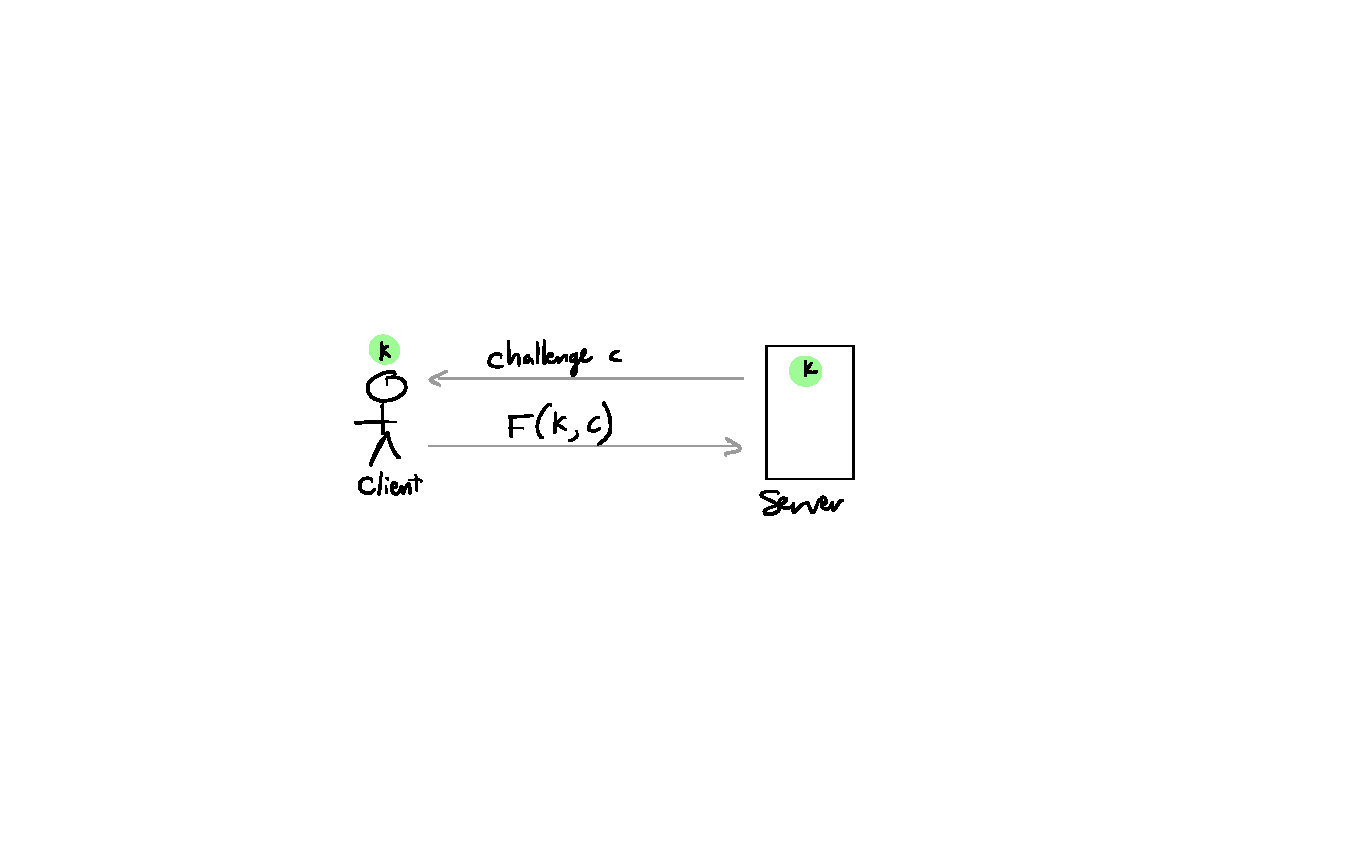
\includegraphics[width=0.8\textwidth]{figs/auth-eavesdropping.pdf}
  \caption{A challenge-response-based authentication system. The
  server and client share a secret key $k$. To authenticate, the
  client sends a function $F$ of its secret key and the server's challenge $c$.}\label{fig:auth-eaves}
\end{figure}

\Cref{fig:auth-eaves} describes an \"uber-simplified challenge-response
authentication scheme that provides security against eavesdropping attacks.
The protocol takes place between a client and server holding a shared secret key $k$.
\begin{enumerate}
	\item The server chooses a long random string~$c$, which we call a \textit{challenge} 
        and sends it to the authenticating client.
  \item The client computes an authentication ``tag'' $t \gets F(k, c)$, where $F(\cdot, c)$ is hard to compute without knowing $k$.
        (The function $F$ here is a Message Authentication Code, 
        which we will talk more specifically about in \cref{lec:mac}.)
        The sends the MAC tag $t$ to the server.
  \item The server receives a tag $t'$ from the client and ensures that $t' = F(k,c)$.
        If so, the server considers the authentication successful.
\end{enumerate}
The security of this scheme derives from the fact that an attacker cannot
produce tags $F(k,c)$ on new challenge values $c$. (An attacker can always
try to replay an old tag it has seen, but since the challenge changes with
every authentication request, the server will always reject the old tag.)

\subsection{Time-based One-Time Passwords (TOTP)}
Time-based one-time passwords are a type of challenge-response authentication
protocol. The only difference from \cref{fig:auth-eaves} is that in a TOTP
scheme, the client and server derive the challenge from the current time.
The user has a device, such as 
a phone, that shares a secret key $k$ (e.g., a random 128-bit string) 
with the server.
Both parties agree on a protocol by which to
generate this code---something like $F(k, \texttt{gettimeofday() / 30})$.
The phone can generate the code, display it to the user, and the server
can then verify the code by recomputing it.


\subsection{Authenticating requests}
Often, a client will want to send an \emph{authenticated message} to a server.
That is, the client often wants to simultaneously authenticate to the server
and send a request $\mathsf{req}$, such as $\mathsf{req} = \ttt{rm file.txt}$.
To accomplish this, the client can compute the challenge value as 
the hash of the server-provided challenge $c$ and the client's request.
So the tag looks like:
$t_{\mathsf{req}} \gets F(k, c \| \mathsf{req})$.
Then the client sends the pair $(t_{\mathsf{req}}, \mathsf{req})$ to the server.
In this way, the server can simultaneously authenticate the client
and be sure that the request $\mathsf{req}$ came from the client.

An \textbf{unsafe} way for the client to simultaneously authenticate to the 
server and send a request would be for the client to compute the MAC tag $t \gets \MAC(k,r)$
and then send $(t, \mathsf{req})$ to the server.
A network attacker could modify the client's request to $(t, \mathsf{req'})$ en
route to the server without the server being able to detect this attack.

\subsection{Phishing attacks (attacker-in-the-middle attacks)}
A \emph{phishing} attack is one
in which an attacker tricks a user into giving away their Gmail password,
for example, by creating a website that looks, for example, like the \ttt{gmail.com}
login page.
TOTP passwords have a similar vulnerability:
an attacker can simply ask the user
to give her the one-time code by pretend to be
tech support, or the user's employer, or
a customer-service representative.
In this setting, TOTP 
codes are slightly better than standard passwords since the attacker
must use a stolen TOTP code within $\approx$30 seconds of stealing
it, which requires a much more sophisticated attack.

Phishing attacks take advantage of the fact that in password- and TOTP-based
authentication schemes, there is no binding between the authentication process
and the server's subsequent communication with the client.
The attacker here doesn't really break the authentication scheme; the
problem is that the authentication scheme didn't authenticate enough.
U2F, which we now discuss, handles that issue.

\section{Protecting against active attacks: Signatures and U2F}
\begin{figure}
\centering
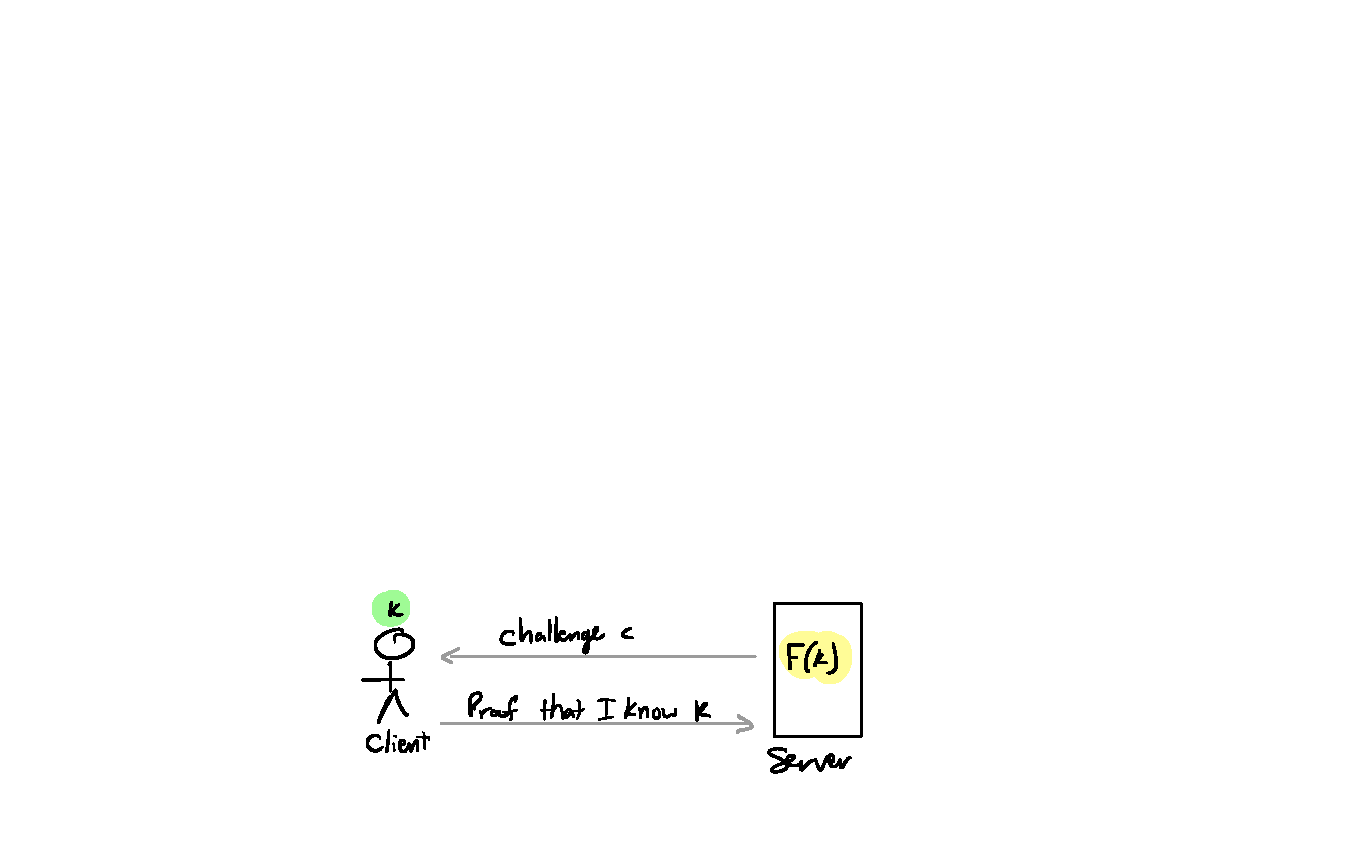
\includegraphics[width=0.7\textwidth]{figs/auth-active.pdf}
\caption{An authentication scheme based on digital signatures.}
\label{fig:auth-active}
\end{figure}

To provide security against active attacks, we can use an authentication
scheme based on digital signatures, which we will discuss in \cref{sec:sig}.
With these schemes, the client has a secret key $k$ and the server stores
some hard-to-invert function of the key $F(k)$.
(We call $F(k)$ the ``public key.'')
In particular, the server \emph{does not store any secrets}---even if the attacker
can compromise the server and/or interact with the honest client, it cannot learn the client's secret key $k$
nor learn any information that it can use to later authenticate as the client.
To authenticate, the server sends the client a challenge and the client produces
a digital signature on the challenge $c$---essentially a proof that the client knows the 
secret key $k$ and that it intended to sign the challenge~$c$.

The U2F USB security tokens that you may have seen use this form of authentication.
As an added bonus, they prevent phishing attacks by binding the authentication process
to the name of the server that the client is trying to authenticate to.
In particular, the U2F software on the client passes the name of the server (e.g., \ttt{amazon.com}),
in addition to a server-provided random challenge $c$, to the U2F token.
The token then produces a signature on the string $c\|\ttt{amazon.com}$.
If the attacker sets up \ttt{amason.com} and gets the user to visit it,
the U2F device will only generate a code that is good for \ttt{amason.com}
and not the real \ttt{amazon.com}. 



\section{Two-Factor Authentication}

Many systems use multiple forms of authentication to try to boost security. 
In particular, as we have already seen, passwords are a weak authentication
mechanism: humans are bad at choosing strong passwords and 
attackers have become good at stealing password databases
and recovering many users' passwords at once.

A common technique to harden password-based authentication systems
is to combine passwords with a second method of 
authentication---one with a different failure mode. 
Common authentication schemes are:

\begin{itemize}
	\item Something you know: password, PIN, etc
	\item Something you have: USB key, phone, etc
	\item Something you are: biometrics (fingerprint, face ID)...
\end{itemize}


